
\providecommand{\Cat}{\mathcal{C}at}
\providecommand{\qcOne}{\mathbf{1}}  %
\providecommand{\hTwoCell}[5]{\tikz[baseline=-0.8ex]{%
  \node (rvl) at (0,0) {$#1$};
  \node (rvr) at (2.9,0) {$#2$};
  \draw[->] (rvl) to[bend left=28] node[above]{$\scriptstyle #3$} (rvr);
  \draw[->] (rvl) to[bend right=28] node[below]{$\scriptstyle #5$} (rvr);
  \node at (1.45,0) {$\scriptstyle #4$};}}
\providecommand{\rvIntCat}[3]{\begin{tikzpicture}[x=1.9em,y=1.4em]%
  \node (rva) at (0,1.1) {$#1$};
  \node (rvb) at (4.8,1.1) {$#2$};
  \node (rvc) at (8.8,1.1) {$#3$};
  \draw[->] (rva) -- node[above]{$\scriptstyle\circ$} (rvb);
  \draw[->] ([yshift=0.42em]rvb) -- node[above]{$\scriptstyle d$} ([yshift=0.42em]rvc);
  \draw[->] (rvc) -- node[below]{$\scriptstyle i$} (rvb);
  \draw[->] ([yshift=-0.62em]rvb) -- node[below]{$\scriptstyle c$} ([yshift=-0.62em]rvc);
\end{tikzpicture}}

\trEnrichedCategory{}论的一个重要特例，出现在以\trCategory{}自身这一%
\trCartesianClosed{}\trCategory{}为富集之基时。\emph{富集于} $\Cat$ 中的%
\trCategory{}——\emph{2-\trCategory}——以及\emph{内部}于 $\Cat$ 定义的%
\trCategory{}——\emph{\trDoubleCategory}——由 Charles Ehresmann 首先引入。
一篇著名的早期综述见于 \cite{bib70}，而全面的现代论述则包括 \cite{bib73} 与%
\cite{bib59}。基本定义在 B.1 节中给出，该节特别关注 2-\trCategory{}中%
2-\trCell{}借助\emph{\trPastingDiagram}（pasting diagrams）进行的复合。

在 B.2 节中，我们简短地回答一个问题：诸 2-\trCategory{}构成什么？我们定义
2-\trCategory{}之间态射的三个维度——\trTwoFunctor、2-\trNaturalTransformation{}%
与\trModification{}（modification）——并观察到这三者全体组装成一个\emph{3-\trCategory}
（3-category），即一个富集于诸 2-\trCategory{}的\trCartesianClosed{}\trCategory{}%
之上的\trCategory。

2-\trCategory{}理论的许多面向都落在\trEnrichedCategory{}论的视野之外。我们在
B.3 节中遇到其中一些：在那里我们发展任意 2-\trCategory{}中的伴随与\trMate{}%
（mates）的演算，以补足 §2.1 的诸结果；并在 B.4 节中研究右伴随右逆伴随这一
特例。在 B.5 节中，我们证明一条引理，它产出被任何\trTwoFunctor{}保持的绝对%
\trLifting{}图。最后，在 B.6 节中我们考虑各种 2-范畴论结构的可表示性，并
简短评论\trBicategorical{} Yoneda 引理。

\section{2-\trCategory{}与\trPastingDiagram{}演算}\label{sec:two-categories-and-the-calculus-of-pasting-diagrams}

小\trCategory{}的\trCategory{} $\Cat$ 是\trCartesianClosed：指数 $B^{A}$
定义为从 $A$ 到 $B$ 的\trFunctor{}与\trNaturalTransformation{}的\trCategory，
而\trTerminal{}对象则由终范畴 $\qcOne$ 给出。利用附录 A 中的工作，我们可以
简洁地把一个 2-\trCategory{}定义为富集于这个\trCartesianClosed{}\trCategory{}%
之上的一个\trCategory。附录 A 中的\cref{lem:cartesian-closed-v-category}随即
给出第一个例子：由于任何\trCartesianClosed{}\trCategory{}都富集于其自身之上，
$\Cat$ 定义了 2-\trCategory{}的一个例子——原型性的例子。

拆解附录 A 中的\cref{def:enriched-category}，我们看到一个 2-\trCategory{}%
包含了相当多的结构：

\begin{definition}[2-\trCategory]\label{def:two-category}
一个 \textbf{2-\trCategory} $\mathcal{C}$ 是富集于 $\Cat$ 中的一个%
\trCategory。显式地，它拥有：
\begin{itemize}
\item 对象的一个汇集；
\item 对每一对对象 $a$，$b\in\mathcal{C}$，一个由箭头 $f\colon a\to b$
  组成的汇集，这些箭头亦称作 \textbf{1-\trCell}，它们是 hom-\trCategory{}
  $\mathcal{C}(a,b)$ 的对象；并且
\item 对每一对 1-\trCell{} $f$，$g\colon a\to b$，一个由箭头之间的箭头
  \hTwoCell{a}{b}{f}{\Downarrow\alpha}{g} 组成的汇集，称为
  \textbf{2-\trCell}，\footnote{在这种图示表示中，隐含地要求一个
  2-\trCell{} $\alpha$ 具有定义域 1-\trCell{} $f$ 与余定义域 1-\trCell{}
  $g$，而这两支 1-\trCell{}拥有公共的定义域对象 $a$ 与余定义域对象 $b$——
  它们即 $\alpha$ 的源 0-\trCell{}与靶 0-\trCell。}这些 2-\trCell{}即
  hom-\trCategory{} $\mathcal{C}(a,b)$ 中从 $f$ 到 $g$ 的诸态射
  $\alpha\colon f\Rightarrow g$。
\end{itemize}
使得：
\begin{enumerate}[label=(\roman*)]
\item 对每一对固定的对象 $a$，$b\in\mathcal{C}$，诸 1-\trCell{}与诸
  2-\trCell{}构成一个\trCategory。特别地：
  \begin{itemize}
  \item 如下左图的一对 2-\trCell{}容有如下右图所示的一个\textbf{竖直复合}
    （vertical composite）：
    \begin{center}
    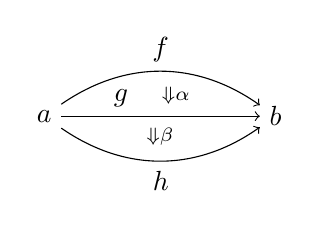
\begin{tikzpicture}[x=1.9em,y=1.35em]
      \node (a) at (0,0) {$a$};
      \node (b) at (4.4,0) {$b$};
      \draw[->] (a) to[bend left=35] node[above]{$f$} (b);
      \draw[->] (a) -- node[above,pos=0.3]{$g$} (b);
      \draw[->] (a) to[bend right=35] node[below]{$h$} (b);
      \node at (2.5,0.55) {$\scriptstyle\Downarrow\alpha$};
      \node at (2.2,-0.55) {$\scriptstyle\Downarrow\beta$};
    \end{tikzpicture}
    $\;=:\;$
    \hTwoCell{a}{b}{f}{\Downarrow\beta\cdot\alpha}{h}
    \end{center}
  \item 每支 1-\trCell{} $f\colon a\to b$ 都拥有一个恒等 2-\trCell{}
    \hTwoCell{a}{b}{f}{\Downarrow\mathrm{id}_f}{f}。
  \end{itemize}
\item 诸对象与诸 1-\trCell{}按通常的意义定义一个\trCategory；特别地，每个
  对象都拥有恒等箭头 $\mathrm{id}_{a}\colon a\to a$。
\item 诸对象与诸 2-\trCell{}构成一个\trCategory。特别地：
  \begin{itemize}
  \item 如下左图的一对 2-\trCell{}容有一个\textbf{水平复合}（horizontal
    composite），如下右图所示：
    \begin{center}
    \hTwoCell{a}{b}{f}{\Downarrow\alpha}{g}
    \hTwoCell{b}{c}{j}{\Downarrow\gamma}{k}
    $\;=:\;$
    \hTwoCell{a}{c}{jf}{\Downarrow\gamma\ast\alpha}{kg}
    \end{center}
  \item 恒等 1-\trCell{}上的恒等 2-\trCell{}
    \hTwoCell{a}{a}{\mathrm{id}_a}{\Downarrow\mathrm{id}_{\mathrm{id}_a}}{\mathrm{id}_a}
    定义水平复合的单位。
  \end{itemize}
\item 最后，水平复合相对竖直复合是函子式的：
  \begin{itemize}
  \item 恒等 2-\trCell{}的水平复合物是恒等 2-\trCell{}：
    \begin{center}
    \hTwoCell{a}{b}{g}{\Downarrow\mathrm{id}_g}{g}
    \hTwoCell{b}{c}{k}{\Downarrow\mathrm{id}_k}{k}
    $\;=\;$%
    \hTwoCell{a}{c}{kg}{\Downarrow\mathrm{id}_{kg}}{kg}
    \end{center}
  \item 在下述情形中，诸竖直复合物的水平复合与诸水平复合物的竖直复合相
    重合，这一性质被称为\textbf{中四交换}（middle-four interchange）：
    \begin{center}
    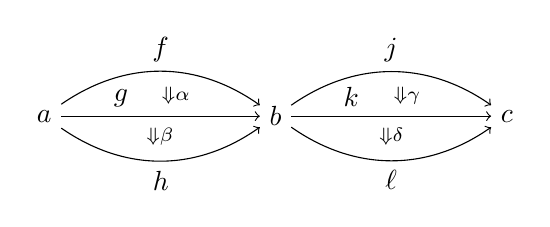
\begin{tikzpicture}[x=1.9em,y=1.35em]
      \node (a) at (0,0) {$a$};
      \node (b) at (4.4,0) {$b$};
      \node (c) at (8.8,0) {$c$};
      \draw[->] (a) to[bend left=35] node[above]{$f$} (b);
      \draw[->] (a) -- node[above,pos=0.3]{$g$} (b);
      \draw[->] (a) to[bend right=35] node[below]{$h$} (b);
      \node at (2.5,0.55) {$\scriptstyle\Downarrow\alpha$};
      \node at (2.2,-0.55) {$\scriptstyle\Downarrow\beta$};
      \draw[->] (b) to[bend left=35] node[above]{$j$} (c);
      \draw[->] (b) -- node[above,pos=0.3]{$k$} (c);
      \draw[->] (b) to[bend right=35] node[below]{$\ell$} (c);
      \node at (6.9,0.55) {$\scriptstyle\Downarrow\gamma$};
      \node at (6.6,-0.55) {$\scriptstyle\Downarrow\delta$};
    \end{tikzpicture}
    \quad
    $(\delta\ast\beta)\cdot(\gamma\ast\alpha)=(\delta\cdot\gamma)\ast(\beta\cdot\alpha)$
    \end{center}
  \end{itemize}
\end{enumerate}
\end{definition}

水平复合的一个退化特例——其中除一个 2-\trCell{}之外，其余的 2-\trCell{}都是
其边缘 1-\trCell{} $f$ 上的恒等 $\mathrm{id}_{f}$——被称为「\trWhiskering」。

\begin{definition}[\trWhiskering]\label{def:whiskering}
一个 2-\trCell{} \hTwoCell{a}{b}{f}{\Downarrow\alpha}{g} 与一对 1-\trCell{}
$k\colon x\to a$ 及 $h\colon b\to y$ 的\textbf{须状复合}（whiskered
composite）$h\alpha k$ 定义为水平复合：
\begin{center}
\hTwoCell{x}{y}{hfk}{\Downarrow h\alpha k}{hgk}
$\;:=\;$
\begin{tikzpicture}[x=1.9em,y=1.35em]
  \node (x) at (0,0) {$x$};
  \node (a) at (2.8,0) {$a$};
  \node (b) at (6.4,0) {$b$};
  \node (y) at (9.4,0) {$y$};
  \draw[->] (x) -- node[above]{$k$} (a);
  \draw[->] (a) to[bend left=30] node[above]{$f$} (b);
  \draw[->] (a) to[bend right=30] node[below]{$g$} (b);
  \node at (4.6,0) {$\scriptstyle\Downarrow\alpha$};
  \draw[->] (b) -- node[above]{$h$} (y);
\end{tikzpicture}
\\[0.5em]
$\;:=\;$
\hTwoCell{x}{a}{k}{\Downarrow\mathrm{id}_k}{k}
\hTwoCell{a}{b}{f}{\Downarrow\alpha}{g}
\hTwoCell{b}{y}{h}{\Downarrow\mathrm{id}_h}{h}
\end{center}
\end{definition}

正如下面的引理所揭示的，水平复合可以从竖直复合与\trWhiskering{}中恢复出来。
然而，我们对这一结果的主要兴趣却在于作为陈述最后一部分出现的一个相当平淡的
推论——它出人意料地经常恰其所用。

\begin{lemma}[\trWhiskering{}的自然性]\label{lem:naturality-of-whiskering}
对 2-\trCategory{}中任何可水平复合的 2-\trCell{}对，在从其定义域对象到余
定义域对象的 hom-\trCategory{}中，存在一个由诸须状胞腔组成的交换方块，其对
角线定义水平复合：
\begin{center}
$\mathcal{C}\ni$
\hTwoCell{a}{b}{f}{\Downarrow\alpha}{g}
\hTwoCell{b}{c}{h}{\Downarrow\beta}{k}
$\;\rightsquigarrow\;$
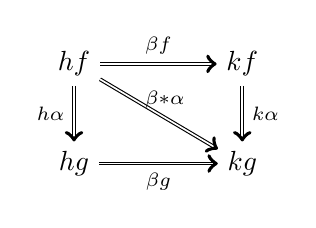
\begin{tikzpicture}[x=1.9em,y=1.5em]
  \node (hf) at (0,1.2) {$hf$};
  \node (kf) at (3.2,1.2) {$kf$};
  \node (hg) at (0,-1.2) {$hg$};
  \node (kg) at (3.2,-1.2) {$kg$};
  \draw[double,->] (hf) -- node[above]{$\scriptstyle\beta f$} (kf);
  \draw[double,->] (hf) -- node[left]{$\scriptstyle h\alpha$} (hg);
  \draw[double,->] (kf) -- node[right]{$\scriptstyle k\alpha$} (kg);
  \draw[double,->] (hg) -- node[below]{$\scriptstyle\beta g$} (kg);
  \draw[double,->] (hf) -- node[above,pos=0.55]{$\scriptstyle\beta\ast\alpha$} (kg);
\end{tikzpicture}
$\;\in\mathcal{C}(a,c)$
\end{center}
特别地，四枚须状 2-\trCell{} $h\alpha$、$k\alpha$、$\beta f$ 与 $\beta g$
中若有任何三枚可逆，则第四枚亦可逆。
\end{lemma}

\begin{proof}
由中四交换：
\begin{align*}
\beta g\cdot h\alpha
  &= (\beta\ast\mathrm{id}_g)\cdot(\mathrm{id}_h\ast\alpha)
   = (\beta\cdot\mathrm{id}_h)\ast(\mathrm{id}_g\cdot\alpha)
   = \beta\ast\alpha\\
  &= (\mathrm{id}_k\cdot\beta)\ast(\alpha\cdot\mathrm{id}_f)
   = (\mathrm{id}_k\ast\alpha)\cdot(\beta\ast\mathrm{id}_f)
   = k\alpha\cdot\beta f.
\end{align*}
\end{proof}

水平复合与竖直复合这两种操作，都是经\emph{粘贴}（pasting）而复合的特例，
后者由 Bénabou 首先引入 \cite{bib9}。其主要结果——在 2-范畴论语境中由
Power 证明 \cite{bib91}——是说，一张如下方这样良构的\trPastingDiagram{}拥有
唯一的 2-\trCell{}复合物：\footnote{此结果由\trVerity{}推广到弱 2-范畴论
语境 \cite{bib130}，在后一情形下，一旦指明其源 1-\trCell{}与靶 1-\trCell，
复合 2-\trCell{}便是良定义的（另见 \cite{bib58}）。}

\begin{rveq}\label{eq:pasting-diagram}
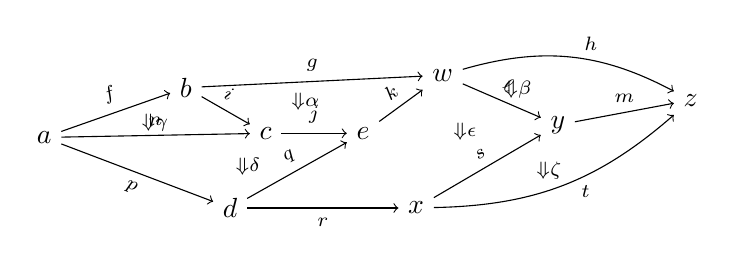
\begin{tikzpicture}[x=1.6em,y=1.5em]
  \node (a) at (0,0)      {$a$};
  \node (b) at (3.2,1.2)  {$b$};
  \node (w) at (9.0,1.5)  {$w$};
  \node (c) at (5.0,0.1)  {$c$};
  \node (e) at (7.2,0.1)  {$e$};
  \node (y) at (11.6,0.3) {$y$};
  \node (z) at (14.6,0.9) {$z$};
  \node (d) at (4.2,-1.7) {$d$};
  \node (x) at (8.4,-1.7) {$x$};
  \draw[->] (a) -- node[above,sloped]{$\scriptstyle f$} (b);
  \draw[->] (b) -- node[above]{$\scriptstyle g$} (w);
  \draw[->] (w) to[bend left=22] node[above,pos=0.6]{$\scriptstyle h$} (z);
  \draw[->] (b) -- node[above,sloped,pos=0.4]{$\scriptstyle i$} (c);
  \draw[->] (c) -- node[above]{$\scriptstyle j$} (e);
  \draw[->] (e) -- node[above,sloped]{$\scriptstyle k$} (w);
  \draw[->] (w) -- node[above,sloped]{$\scriptstyle\ell$} (y);
  \draw[->] (y) -- node[above]{$\scriptstyle m$} (z);
  \draw[->] (a) -- node[above]{$\scriptstyle n$} (c);
  \draw[->] (a) -- node[below,sloped]{$\scriptstyle p$} (d);
  \draw[->] (d) -- node[above,sloped]{$\scriptstyle q$} (e);
  \draw[->] (d) -- node[below]{$\scriptstyle r$} (x);
  \draw[->] (x) -- node[above,sloped]{$\scriptstyle s$} (y);
  \draw[->] (x) to[bend right=20] node[below,pos=0.6]{$\scriptstyle t$} (z);
  \node at (2.5,0.35)  {$\scriptstyle\Downarrow\gamma$};
  \node at (5.9,0.85)  {$\scriptstyle\Downarrow\alpha$};
  \node at (4.6,-0.7)  {$\scriptstyle\Downarrow\delta$};
  \node at (9.5,0.15)  {$\scriptstyle\Downarrow\epsilon$};
  \node at (10.7,1.15) {$\scriptstyle\Downarrow\beta$};
  \node at (11.4,-0.8) {$\scriptstyle\Downarrow\zeta$};
\end{tikzpicture}
\end{rveq}

我们将这一结果的形式陈述与证明留给文献，转而非正式地描述这类粘贴复合物应当
如何解读。

\begin{digression}[如何读取一张\trPastingDiagram]\label{dig:how-to-read-a-pasting-diagram}
2-\trCategory{} $\mathcal{C}$ 中的一张\trPastingDiagram{}表示一个唯一的复合
2-\trCell，它在对象对之间的某个 hom-\trCategory{}中定义一个态射。为了辨认
这些对象，考察\trPastingDiagram{}中对象与 1-\trCell{}的底有向图。若该%
\trPastingDiagram{}是良构的，这个图将拥有唯一的源对象 $a$ 与唯一的靶对象
$z$。这表明\trPastingDiagram{}在 hom-\trCategory{} $\mathcal{C}(a,z)$ 中
定义一个 2-\trCell。对象 $a$ 是它的\textbf{源 0-\trCell}（source 0-cell），
对象 $z$ 是它的\textbf{靶 0-\trCell}（target 0-cell）。

下一步是辨认\trPastingDiagram{}的\textbf{源 1-\trCell}（source 1-cell）与
\textbf{靶 1-\trCell}（target 1-cell）。二者都将是 $\mathcal{C}(a,z)$ 的
对象，即 2-\trCategory{}中从 $a$ 到 $z$ 的 1-\trCell。同样，若%
\trPastingDiagram{}是良构的，源 1-\trCell{}将是唯一的、由 1-\trCell{}组成的
可复合路径，其中没有任何一支作为\trPastingDiagram{}中任何 2-\trCell{}的余
定义域的一部分出现。在 \eqref{eq:pasting-diagram} 中，这些是标签出现在箭头
上方的那些 1-\trCell，其复合为 $hgf$。对偶地，靶 1-\trCell{}将是唯一的、由
1-\trCell{}组成的可复合路径，其中没有任何一支作为\trPastingDiagram{}中任何
2-\trCell{}的定义域的一部分出现。在 \eqref{eq:pasting-diagram} 中，这些是
标签出现在图表下方的那些 1-\trCell，其复合为 $trp$。

最后一步是把\trPastingDiagram{}表示为一个从 $a$ 到 $z$ 的 2-\trCell{}竖直
复合，其中每个 2-\trCell{}都是所示「原子」2-\trCell{}之一的须状复合。诸须状
原子 2-\trCell{}的源与靶描出从 $a$ 到 $z$、穿过\trPastingDiagram{}底有向图
的可复合路径，这些路径彼此仅相差「把原子 2-\trCell{}的源替换为它的靶」这一
步。\trPastingDiagram{}中的每个 2-\trCell{}都将恰好标记该复合的诸
2-\trCell{}中的一个。这些竖直 2-\trCell{}复合的表达式未必唯一，也未必穿过
每条可能的 1-\trCell{}可复合路径，不过总存在某个 2-\trCell{}的竖直复合穿过
每条 1-\trCell{}路径。

首先，在\trPastingDiagram{}中任选一个 2-\trCell，其 1-\trCell{}源可以在源
1-\trCell{}中作为一个子序列被找到；在 \eqref{eq:pasting-diagram} 中，
$\alpha$ 或 $\beta$ 皆可选作第一个。对它作\trWhiskering，使之定义一个从源
1-\trCell{} $hgf$ 到另一条从 $a$ 到 $z$、穿过该\trPastingDiagram{}的可复合
1-\trCell{}路径的 2-\trCell。于是这个须状复合便构成诸可复合 2-\trCell{}序列
的第一步。将\trPastingDiagram{}的这一部分移去并重复，直至抵达靶 1-\trCell。
在上面的例子中，共有四种可能的方式把复合粘贴胞腔 \eqref{eq:pasting-diagram}
表达为须状 2-\trCell{}的竖直复合，它们由 $\mathcal{C}(a,z)$ 中如下交换图表
的四条路径所表示：\footnote{原书此图表底行第二节点及其入边（自 $m\ell gf$ 右
行之边）的标签印作「$m\ell kjia$」与「$m\ell\alpha a$」，其末字符 $a$ 系源
0-\trCell，缀于 1-\trCell{}复合路径之末于数学不通；按顶行对应节点（$hkjif$）
与竖直边标签（$\beta kjif$）当为 $f$，此处径改。——译者注}
\begin{center}
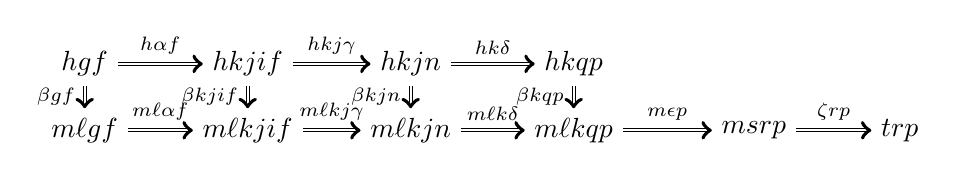
\begin{tikzpicture}[x=1.55em,y=1.6em]
  \node (t1) at (0,1.5)    {$hgf$};
  \node (t2) at (3.8,1.5)  {$hkjif$};
  \node (t3) at (7.6,1.5)  {$hkjn$};
  \node (t4) at (11.4,1.5) {$hkqp$};
  \node (b1) at (0,0)      {$m\ell gf$};
  \node (b2) at (3.8,0)    {$m\ell kjif$};
  \node (b3) at (7.6,0)    {$m\ell kjn$};
  \node (b4) at (11.4,0)   {$m\ell kqp$};
  \node (b5) at (15.6,0)   {$msrp$};
  \node (b6) at (19.0,0)   {$trp$};
  \draw[double,->] (t1) -- node[above]{$\scriptstyle h\alpha f$} (t2);
  \draw[double,->] (t2) -- node[above]{$\scriptstyle hkj\gamma$} (t3);
  \draw[double,->] (t3) -- node[above]{$\scriptstyle hk\delta$} (t4);
  \draw[double,->] (t1) -- node[left]{$\scriptstyle\beta gf$} (b1);
  \draw[double,->] (t2) -- node[left]{$\scriptstyle\beta kjif$} (b2);
  \draw[double,->] (t3) -- node[left]{$\scriptstyle\beta kjn$} (b3);
  \draw[double,->] (t4) -- node[left]{$\scriptstyle\beta kqp$} (b4);
  \draw[double,->] (b1) -- node[above]{$\scriptstyle m\ell\alpha f$} (b2);
  \draw[double,->] (b2) -- node[above]{$\scriptstyle m\ell kj\gamma$} (b3);
  \draw[double,->] (b3) -- node[above]{$\scriptstyle m\ell k\delta$} (b4);
  \draw[double,->] (b4) -- node[above]{$\scriptstyle m\epsilon p$} (b5);
  \draw[double,->] (b5) -- node[above]{$\scriptstyle\zeta rp$} (b6);
\end{tikzpicture}
\end{center}
\end{digression}

一个 2-\trCategory{}共有四个对偶（含其自身），每一者都与它拥有相同的对象、
1-\trCell{}与 2-\trCell，但会在某个维度上交换定义域与余定义域。

\begin{definition}[op-对偶与 co-对偶]\label{def:op-co-duals}
设 $\mathcal{C}$ 为一个 2-\trCategory。
\begin{itemize}
\item 它的 \textbf{op-对偶}（op-dual）$\mathcal{C}^{\mathrm{op}}$ 是满足
  $\mathcal{C}^{\mathrm{op}}(a,b):=\mathcal{C}(b,a)$ 的 2-\trCategory。它
  反转 1-\trCell{}的方向，但不反转 2-\trCell{}的方向。
\item 它的 \textbf{co-对偶}（co-dual）$\mathcal{C}^{\mathrm{co}}$ 是满足
  $\mathcal{C}^{\mathrm{co}}(a,b):=\mathcal{C}(a,b)^{\mathrm{op}}$ 的
  2-\trCategory。它反转 2-\trCell{}的方向，但不反转 1-\trCell{}的方向。
\item 它的 \textbf{coop-对偶}（coop-dual）$\mathcal{C}^{\mathrm{coop}}$ 是
  满足 $\mathcal{C}^{\mathrm{coop}}(a,b):=\mathcal{C}(b,a)^{\mathrm{op}}$
  的 2-\trCategory。它同时反转 2-\trCell{}与 1-\trCell{}的方向。
\end{itemize}
\end{definition}

我们从第 1 章中的\cref{def:equivalence-2-category}回忆起：一个 2-\trCategory{}%
中的\trEquivalence{}由下列数据给出：
\begin{itemize}
\item 一对对象 $a$ 与 $b$；
\item 一对 1-\trCell{} $f\colon a\to b$ 与 $g\colon b\to a$；
\item 一对可逆 2-\trCell\footnote{对 2-\trCell{}而言，「可逆性」的默认含义
  是对竖直复合可逆。注意，一个可逆 2-\trCell{}的边缘 1-\trCell{}未必可逆。}
  \hTwoCell{a}{a}{\mathrm{id}_a}{\cong\;\Downarrow\alpha}{gf}
  及
  \hTwoCell{b}{b}{fg}{\cong\;\Downarrow\beta}{\mathrm{id}_b}。
\end{itemize}

\begin{digression}[2-\trCategory{}内部的诸「相同」概念]\label{dig:notions-of-sameness}
从 2-范畴论的观点看，对一个 2-\trCategory{}的两个对象而言，最自然的「相同」
概念是\emph{\trEquivalence}：$a$ 与 $b$ 被视作相同的，若二者之间存在一个%
\trEquivalence。

对一个 2-\trCategory{}中一对平行的态射而言，最自然的「相同」概念是%
\emph{\trIsomorphism}：$h$，$k\colon a\to b$ 被视作相同的，若存在一个可逆
2-\trCell{} $\gamma\colon h\cong k$。

对一个具有公共边缘的 2-\trCell{}对而言，最自然的「相同」概念是\emph{相等}。由于
2-\trCategory{}缺乏任何可以在 2-\trCell{}之间作中介的更高维态射，这里没有
更弱的概念可用。
\end{digression}

在第 1 章中的\cref{dig:simplicial-categories}中，我们看到\trSimplicialCategory{}%
的数据可以表达为一个取值于 $\Cat$ 的特定类型的\trDiagram。一个小
2-\trCategory{}可以类似地被编码为——事实上以两种不同的方式——一个定义
\emph{内部}于诸\trCategory{}的\trCategory{}之中的\trCategory。

\begin{definition}[内范畴]\label{def:internal-category}
设 $\mathcal{E}$ 为任一带\trPullback{}的\trCategory。$\mathcal{E}$ 中的一个
\textbf{内范畴}（internal category）由如下数据给出
\begin{center}
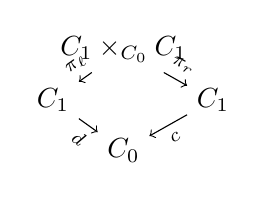
\begin{tikzpicture}[x=1.7em,y=1.3em]
  \node (t) at (1.5,2.2)  {$C_{1}\times_{C_{0}}C_{1}$};
  \node (l) at (0,0.8)    {$C_{1}$};
  \node (r) at (3.4,0.8)  {$C_{1}$};
  \node (b) at (1.5,-0.6) {$C_{0}$};
  \draw[->] (t) -- node[above,sloped]{$\scriptstyle\pi_{\ell}$} (l);
  \draw[->] (t) -- node[above,sloped]{$\scriptstyle\pi_{r}$} (r);
  \draw[->] (l) -- node[below,sloped]{$\scriptstyle d$} (b);
  \draw[->] (r) -- node[below,sloped]{$\scriptstyle c$} (b);
\end{tikzpicture}
\qquad
\rvIntCat{C_{1}\times_{C_{0}}C_{1}}{C_{1}}{C_{0}}
\end{center}
并服从一些交换图表，这些图表定义复合与单位的定义域和余定义域
\begin{center}
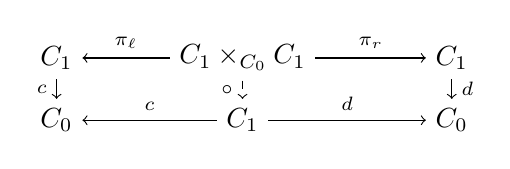
\begin{tikzpicture}[x=2.1em,y=1.5em]
  \node (tl) at (0,1.5)    {$C_{1}$};
  \node (tm) at (3.2,1.5)  {$C_{1}\times_{C_{0}}C_{1}$};
  \node (tr) at (6.8,1.5)  {$C_{1}$};
  \node (bl) at (0,0)      {$C_{0}$};
  \node (bm) at (3.2,0)    {$C_{1}$};
  \node (br) at (6.8,0)    {$C_{0}$};
  \draw[->] (tm) -- node[above]{$\scriptstyle\pi_{\ell}$} (tl);
  \draw[->] (tm) -- node[above]{$\scriptstyle\pi_{r}$} (tr);
  \draw[->] (tl) -- node[left]{$\scriptstyle c$} (bl);
  \draw[->,dashed] (tm) -- node[left]{$\scriptstyle\circ$} (bm);
  \draw[->] (tr) -- node[right]{$\scriptstyle d$} (br);
  \draw[->] (bm) -- node[above]{$\scriptstyle c$} (bl);
  \draw[->] (bm) -- node[above]{$\scriptstyle d$} (br);
\end{tikzpicture}
\qquad
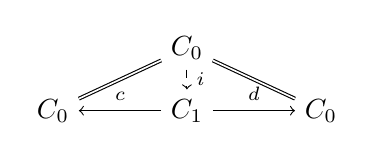
\begin{tikzpicture}[x=2.2em,y=1.5em]
  \node (t)  at (2.2,1.5) {$C_{0}$};
  \node (bl) at (0,0)     {$C_{0}$};
  \node (bm) at (2.2,0)   {$C_{1}$};
  \node (br) at (4.4,0)   {$C_{0}$};
  \draw[double] (t) -- (bl);
  \draw[double] (t) -- (br);
  \draw[->,dashed] (t) -- node[right]{$\scriptstyle i$} (bm);
  \draw[->] (bm) -- node[above]{$\scriptstyle c$} (bl);
  \draw[->] (bm) -- node[above]{$\scriptstyle d$} (br);
\end{tikzpicture}
\end{center}
并编码复合为结合且幺一这一事实。
\begin{center}
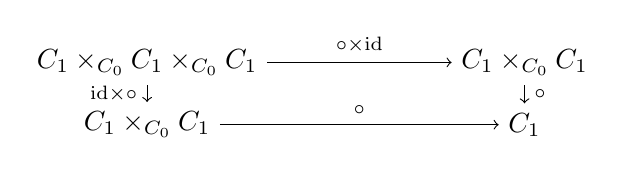
\begin{tikzpicture}[x=2.2em,y=1.5em]
  \node (tl) at (0,1.5)   {$C_{1}\times_{C_{0}}C_{1}\times_{C_{0}}C_{1}$};
  \node (tr) at (6.2,1.5) {$C_{1}\times_{C_{0}}C_{1}$};
  \node (bl) at (0,0)     {$C_{1}\times_{C_{0}}C_{1}$};
  \node (br) at (6.2,0)   {$C_{1}$};
  \draw[->] (tl) -- node[above]{$\scriptstyle\circ\times\mathrm{id}$} (tr);
  \draw[->] (tl) -- node[left]{$\scriptstyle\mathrm{id}\times\circ$} (bl);
  \draw[->] (tr) -- node[right]{$\scriptstyle\circ$} (br);
  \draw[->] (bl) -- node[above]{$\scriptstyle\circ$} (br);
\end{tikzpicture}
\qquad
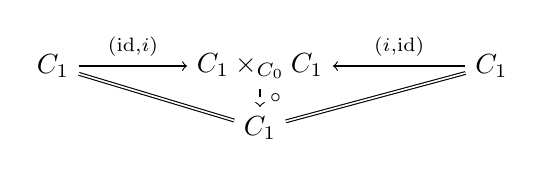
\begin{tikzpicture}[x=2.2em,y=1.5em]
  \node (l) at (0,1.5)    {$C_{1}$};
  \node (t) at (3.4,1.5)  {$C_{1}\times_{C_{0}}C_{1}$};
  \node (r) at (7.2,1.5)  {$C_{1}$};
  \node (b) at (3.4,0)    {$C_{1}$};
  \draw[->] (l) -- node[above]{$\scriptstyle(\mathrm{id},i)$} (t);
  \draw[->] (r) -- node[above]{$\scriptstyle(i,\mathrm{id})$} (t);
  \draw[->,dashed] (t) -- node[right]{$\scriptstyle\circ$} (b);
  \draw[double] (l) -- (b);
  \draw[double] (r) -- (b);
\end{tikzpicture}
\end{center}
\end{definition}

$\mathcal{S}et$ 中的一个内范畴是一个通常的小\trCategory。$\Cat$ 中的一个
内范畴定义一个\trDoubleCategory：

\begin{definition}[\trDoubleCategory]\label{def:double-category}
一个 \textbf{\trDoubleCategory} $\mathcal{C}$ 是 $\Cat$ 中的一个内范畴
\begin{center}
\rvIntCat{C_{h,s}\times_{C_{o,v}}C_{h,s}}{C_{h,s}}{C_{o,v}}
\end{center}
显式地，它拥有：
\begin{itemize}
\item 一个由对象与\textbf{竖直箭头}（vertical arrows）组成的\trCategory{}
  $C_{o,v}$；
\item 一个由\textbf{水平箭头}（horizontal arrows）与\textbf{方块}
  （squares）组成的\trCategory{} $C_{h,s}$；
\item \trFunctor{} $c$，$d\colon C_{h,s}\to C_{o,v}$，为每支水平箭头指派一
  个余定义域／定义域对象，并为每个方块指派一支余定义域／定义域竖直箭头；
\item \trFunctor{} $i\colon C_{o,v}\to C_{h,s}$，为每个对象指派一支水平恒等
  箭头，并为每支竖直箭头指派一个恒等方块；并且
\item 复合\trFunctor{} $\circ\colon C_{h,s}\times_{C_{o,v}}C_{h,s}\to C_{h,s}$，
  它定义水平箭头与方块的水平复合，且对每个变元处的竖直复合是函子式的
\end{itemize}
满足由内范畴的交换图表所强加的诸公理。
\end{definition}

一个 2-\trCategory{}可以按下列两种方式实现为这一构造的特例。

\begin{digression}[作为范畴对象的 2-\trCategory]\label{dig:two-categories-as-category-objects}
一个 2-\trCategory{}可以被定义为 $\Cat$ 中的一个内范畴
\begin{center}
\rvIntCat{C_{1,2}\times_{C_{0}}C_{1,2}}{C_{1,2}}{C_{0}}
\end{center}
其中\trCategory{} $C_{0}$ 是一个集合，即该 2-\trCategory{}的对象之集。
1-\trCell{}与 2-\trCell{}作为\trCategory{} $C_{1,2}$ 的对象与箭头出现。
\trFunctor{} $d$，$c\colon C_{1,2}\to C_{0}$ 把 1-\trCell{}与 2-\trCell{}送
到各自的定义域 0-\trCell{}与余定义域 0-\trCell。\trFunctor{}
$i\colon C_{0}\to C_{1,2}$ 把每个对象送到它的恒等 1-\trCell。\trFunctor{}
$\circ\colon C_{1,2}\times_{C_{0}}C_{1,2}\to C_{1,2}$ 在对象上的作用定义
1-\trCell{}的复合，而在态射上的作用定义 2-\trCell{}上的水平复合。2-\trCell{}%
上的竖直复合就是\trCategory{} $C_{1,2}$ 内部的复合。这一映射的\trFunctor{}性
编码了中四交换。\footnote{此定义给出了定义 E.2.4 所描述的 $(\infty,1)$-%
\trCategory{}的\trSegalCategories{}模型的动机。}

对偶地，一个 2-\trCategory{}可以被定义为 $\Cat$ 中的一个内范畴
\begin{center}
\rvIntCat{C_{0,2}\times_{C_{0,1}}C_{0,2}}{C_{0,2}}{C_{0,1}}
\end{center}
其中诸\trCategory{} $C_{0,1}$ 与 $C_{0,2}$ 拥有相同的对象之集，且全部四个%
\trFunctor{}都在对象上恒等。这里，公共的对象之集定义 2-\trCategory{}的
对象，而 $C_{0,1}$ 与 $C_{0,2}$ 的箭头分别定义 1-\trCell{}与 2-\trCell。
\trFunctor{} $d$，$c\colon C_{0,2}\to C_{0,1}$ 为一个 2-\trCell{}定义其
定义域 1-\trCell{}与余定义域 1-\trCell，而\trFunctor{}
$\circ\colon C_{0,2}\times_{C_{0,1}}C_{0,2}\to C_{0,2}$ 则编码 2-\trCell{}%
的竖直复合。\trCategory{} $C_{0,2}$ 内部的复合定义 2-\trCell{}的水平复合。
这一映射的\trFunctor{}性编码了中四交换。
\end{digression}

\subsection*{练习}

\begin{exercise}\label{ex:relate-two-category-enriched-structures}
在富集之基为 $\Cat$ 的情形下，将\cref{def:two-category}中逐项列出的诸结构，同%
附录 A 中的\cref{def:enriched-category}中逐项列出的诸结构联系起来。
\end{exercise}

\begin{exercise}\label{ex:duality-involution-double-categories}
在\trDoubleCategory{}上定义一个对偶对合（duality involution），使之交换%
\cref{dig:two-categories-as-category-objects}中出现的一个 2-\trCategory{}作为%
内范畴的两种表述。
\end{exercise}

